%
% ---- PEPA System Models
%

\section{PEPA System Models}
\begin{shaded}
The proposed system will use distributed architectures.  Users will access it from a web-based front end.  Tickets will be stored in a database partitioned across several data nodes.  In between the web servers and database will be a number of worker applications to service user requests, connected to the web servers by some middleware.

For each architecture it will be assumed that the web application will be designed to cope with the required demand, using a cluster of web servers where the throughput is managed using some HTTP Load Balancing algorithm \cite{RN73}, and potentially Elastic Scaling of servers e.g. using the autoscaling features of Amazon Web Services \cite{RN1064} or Microsoft Azure \cite{RN1065}.
\end{shaded}

%
% ---- Simple microservices
%
\subsection{Simple microservices}

There are two separate databases, one for Athletics tickets, one for Cycling.

It's expected that this architecture will lead to isolation of the skewed demand and that the results of testing the model will not be surprising, but that this will provide a useful control for other architectures.

\begin{figure}
	\caption{Simple microservices architecture}
	\centering
	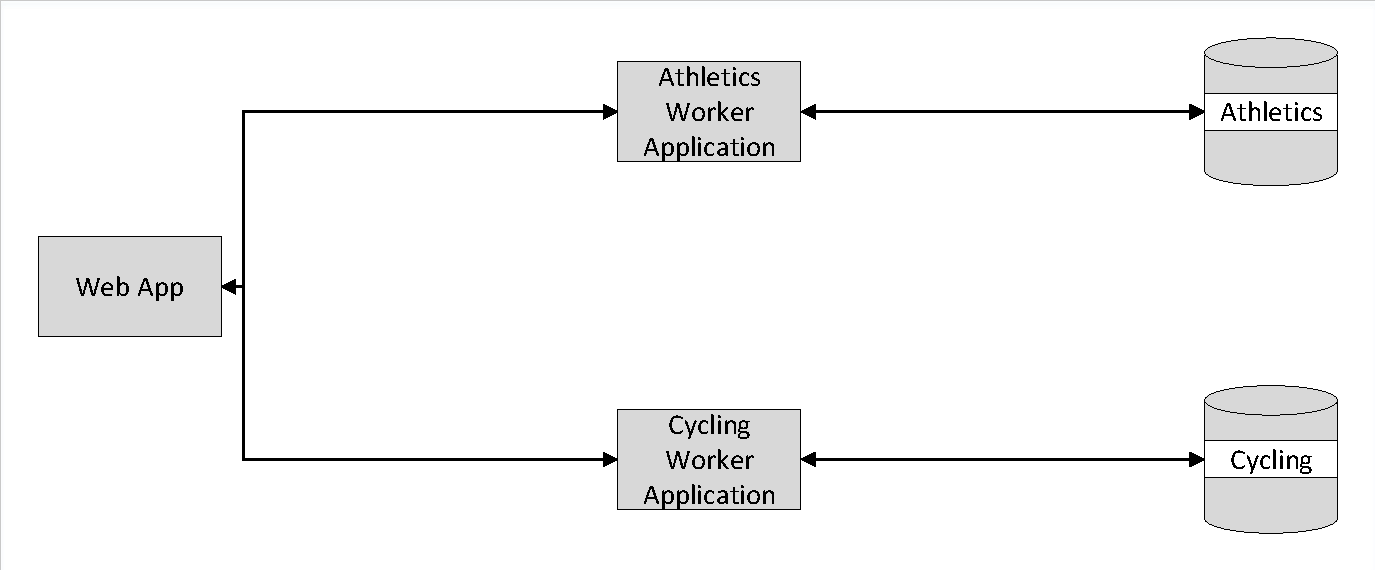
\includegraphics[trim = 5 5 5 5, clip, width=\textwidth]{img/simplemicro}
\end{figure}

\begin{figure}
	\caption{Simple microservices PEPA model}
	\label{figure:simplemicro}
	\centering
	% Automatically generated by PEPA2Latex
	% --begin
	\begin{displaymath}
		\begin{array}{rcl}
			\mathit{a} & = & 1.0 - 10.0\\
			\mathit{c} & = & 1.0\\
			\mathit{w} & = & 100.0\\
			\mathit{db} & = & 6.5\\
			[2.0ex]		\mathit{Website} & \rmdef & (\mathit{athletics},\mathit{a}).\mathit{Website}+(\mathit{cycling},\mathit{c}).\mathit{Website}\\
			\mathit{Worker_A} & \rmdef & (\mathit{athletics},\top).\mathit{WorkerSrv_A}\\
			\mathit{WorkerSrv_A} & \rmdef & (\mathit{workerA},\top).\mathit{Worker_A}\\
			\mathit{Worker_C} & \rmdef & (\mathit{cycling},\top).\mathit{WorkerSrv_C}\\
			\mathit{WorkerSrv_C} & \rmdef & (\mathit{workerC},\top).\mathit{Worker_C}\\
			\mathit{DB_1} & \rmdef & (\mathit{workerA},\mathit{w}).\mathit{DBsrv_1}\\
			\mathit{DBsrv_1} & \rmdef & (\mathit{dbsrv1},\mathit{db}).\mathit{DB_1}\\
			\mathit{DB_2} & \rmdef & (\mathit{workerC},\mathit{w}).\mathit{DBsrv_2}\\
			\mathit{DBsrv_2} & \rmdef & (\mathit{dbsrv2},\mathit{db}).\mathit{DB_2}\\
			\mathit{Service_1} & \rmdef & (\mathit{dbsrv1},\mathit{db}).\mathit{Service_1}\\
			\mathit{Service_2} & \rmdef & (\mathit{dbsrv2},\mathit{db}).\mathit{Service_2}\\
			[2.0ex]		\multicolumn{3}{l}{\mathit{Service_1}\sync{dbsrv1}\mathit{DB_1}\sync{workerA}\mathit{Worker_A}\sync{athletics}\mathit{Website}\sync{cycling}\mathit{Worker_C}\sync{workerC}\mathit{DB_2}\sync{dbsrv2}\mathit{Service_2}}\\
			[2.0ex]	\end{array}
	\end{displaymath}
	% --end
\end{figure}

See the experimental results in Table \ref{table:micro_results}.

\begin{table}[h!]
	\begin{center}
		\caption{Simple microservices experimental results}
		\label{table:micro_results}
		\pgfplotstabletypeset[
		col sep=comma,
		string type,
		columns/a/.style={column name=a, column type={p{.1\textwidth}}},
		columns/athletics/.style={column name=athletics, column type={p{.1\textwidth}}},
		columns/cycling/.style={column name=cycling, column type={p{.1\textwidth}}},
		columns/workerA/.style={column name=workerA, column type={p{.1\textwidth}}},
		columns/workerC/.style={column name=workerC, column type={p{.1\textwidth}}},
		columns/dbsrv1/.style={column name=dbsrv1, column type={p{.1\textwidth}}},
		columns/dbsrv2/.style={column name=dbsrv2, column type={p{.1\textwidth}}},
		every head row/.style={before row=\hline Rate & \multicolumn{6}{c}{Throughput} \\,after row=\hline},
		every last row/.style={after row=\hline},
		]{data/micro/results.csv}
	\end{center}
\end{table}

\begin{figure}
	\caption{Simple microservices experimental results}
	\label{figure:micro_charts}
	\centering
	\begin{tikzpicture}
	\begin{axis}[
	title={Throughput against input rate a},
	xlabel={Rate a},
	ylabel={Throughput},
	xmin=0, xmax=10,
	ymin=0, ymax=7,
	legend pos=north west,
	ymajorgrids=true,
	grid style=dashed,
	cycle multiindex* list={
		mark list*
		\nextlist
		cyan,brown,green,blue,red
	}
	]
	
	\addplot table [x index={0}, y index={1}, col sep=comma]{data/micro/athletics.csv};
	\addplot table [x index={0}, y index={1}, col sep=comma]{data/micro/cycling.csv};
	
	\legend{athletics,cycling}
	
	\end{axis}
	\end{tikzpicture}
\end{figure}

%
% ---- Shared queue and distributed database
%
\subsection{Shared queue and distributed database}

Requests via a shared queue to worker applications going to a distributed database with two nodes, Athletics and Cycling.

\begin{figure}
	\caption{Shared queue middleware architecture}
	\centering
	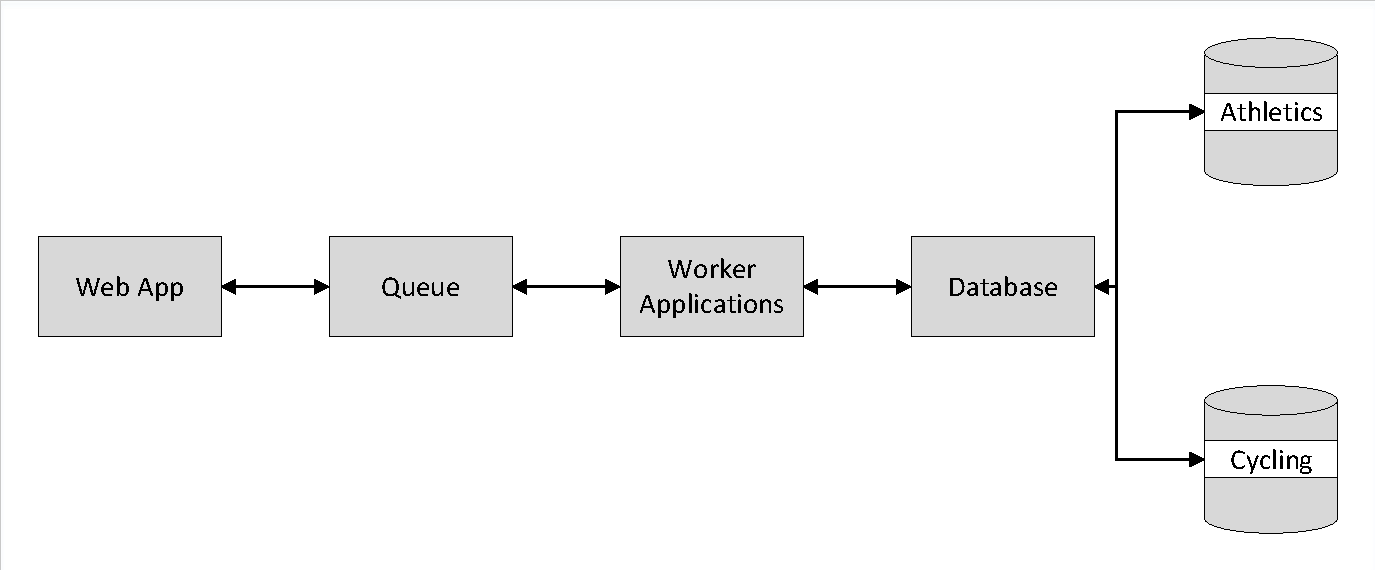
\includegraphics[trim = 5 5 5 5, clip, width=\textwidth]{img/sharedqueue}
\end{figure}

\begin{figure}
	\caption{Shared queue and distributed database}
	\label{figure:queuedd}
	\centering
	% Automatically generated by PEPA2Latex
	% --begin
	\begin{displaymath}
	\begin{array}{rcl}
	\mathit{a} & = & 1.0\\
	\mathit{c} & = & 1.0\\
	\mathit{q} & = & 100.0\\
	\mathit{db} & = & 5.0\\
	[2.0ex]		\mathit{Website} & \rmdef & (\mathit{athletics},\mathit{a}).\mathit{Website}+(\mathit{cycling},\mathit{c}).\mathit{Website}\\
	\mathit{Q_0} & \rmdef & (\mathit{athletics},\top).\mathit{Q_A}+(\mathit{cycling},\top).\mathit{Q_C}\\
	\mathit{Q_A} & \rmdef & (\mathit{queueA},\top).\mathit{Q_0}\\
	\mathit{Q_C} & \rmdef & (\mathit{queueC},\top).\mathit{Q_0}\\
	\mathit{DB_1} & \rmdef & (\mathit{queueA},\mathit{q}).\mathit{DBsrv_1}\\
	\mathit{DBsrv_1} & \rmdef & (\mathit{dbsrv1},\mathit{db}).\mathit{DB_1}\\
	\mathit{DB_2} & \rmdef & (\mathit{queueC},\mathit{q}).\mathit{DBsrv_2}\\
	\mathit{DBsrv_2} & \rmdef & (\mathit{dbsrv2},\mathit{db}).\mathit{DB_2}\\
	\mathit{Service_1} & \rmdef & (\mathit{dbsrv1},\mathit{db}).\mathit{Service_1}\\
	\mathit{Service_2} & \rmdef & (\mathit{dbsrv2},\mathit{db}).\mathit{Service_2}\\
	[2.0ex]		\multicolumn{3}{l}{\mathit{Website}\sync{\substack{athletics\\cycling}}\mathit{Q_0}[N]\sync{\substack{queueA\\queueC}}\mathit{DB_1}\parallel\mathit{DB_2}\sync{\substack{dbsrv1\\dbsrv2}}\mathit{Service_1}\parallel\mathit{Service_2}}\\
	[2.0ex]	\end{array}
	\end{displaymath}
	% --end
\end{figure}

See the experimental results in Table \ref{table:queuedd_results}.

\begin{table}[h!]
	\begin{center}
		\caption{Shared queue and distributed database experimental results}
		\label{table:queuedd_results}
		\pgfplotstabletypeset[
		col sep=comma,
		string type,
		columns/a/.style={column name=a, column type={p{.1\textwidth}}},
		columns/athletics/.style={column name=athletics, column type={p{.1\textwidth}}},
		columns/cycling/.style={column name=cycling, column type={p{.1\textwidth}}},
		columns/qa/.style={column name=queueA, column type={p{.1\textwidth}}},
		columns/qc/.style={column name=queueC, column type={p{.1\textwidth}}},
		columns/dbsrv1/.style={column name=dbsrv1, column type={p{.1\textwidth}}},
		columns/dbsrv2/.style={column name=dbsrv2, column type={p{.1\textwidth}}},
		every head row/.style={before row=\hline Rate & \multicolumn{6}{c}{Throughput} \\,after row=\hline},
		every last row/.style={after row=\hline},
		]{data/qddnr/results.csv}
	\end{center}
\end{table}

%
% ---- Shared queue and distributed database with replication
%
\subsection{Shared queue and distributed database with replication}

Requests via a shared queue to worker applications going to a distributed database with three nodes, Athletics, Cycling and Diving, where each partition is replicated on another node.

\begin{figure}
	\caption{Distributed database with replication architecture}
	\centering
	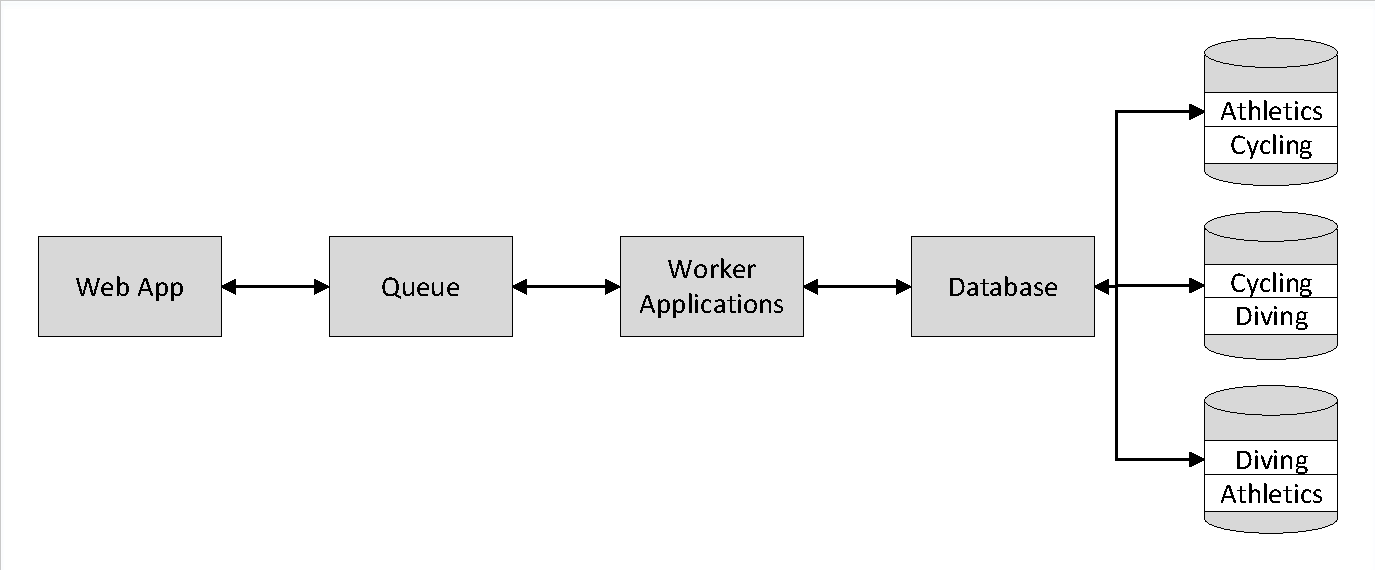
\includegraphics[trim = 5 5 5 5, clip, width=\textwidth]{img/sharedqueue_withrep}
\end{figure}

\begin{figure}
	\caption{Shared queue and distributed database with replication}
	\label{figure:queueddrep}
	\centering
	% Automatically generated by PEPA2Latex
	% --begin
	\begin{displaymath}
	\begin{array}{rcl}
	\mathit{a} & = & 1.0\\
	\mathit{c} & = & 1.0\\
	\mathit{d} & = & 1.0\\
	\mathit{q} & = & 100.0\\
	\mathit{db} & = & 5.0\\
	[2.0ex]		\mathit{Website} & \rmdef & (\mathit{athletics},\mathit{a}).\mathit{Website}+(\mathit{cycling},\mathit{c}).\mathit{Website}+(\mathit{diving},\mathit{d}).\mathit{Website}\\
	\mathit{Q_0} & \rmdef & (\mathit{athletics},\top).\mathit{Q_A}+(\mathit{cycling},\top).\mathit{Q_C}+(\mathit{diving},\top).\mathit{Q_D}\\
	\mathit{Q_A} & \rmdef & (\mathit{queueA},\top).\mathit{Q_0}\\
	\mathit{Q_C} & \rmdef & (\mathit{queueC},\top).\mathit{Q_0}\\
	\mathit{Q_D} & \rmdef & (\mathit{queueD},\top).\mathit{Q_0}\\
	\mathit{DB_1} & \rmdef & (\mathit{queueA},\mathit{q}).\mathit{DBsrv_1}+(\mathit{queueC},\mathit{q}).\mathit{DBsrv_1}\\
	\mathit{DBsrv_1} & \rmdef & (\mathit{dbsrv1},\top).\mathit{DB_1}\\
	\mathit{DB_2} & \rmdef & (\mathit{queueC},\mathit{q}).\mathit{DBsrv_2}+(\mathit{queueD},\mathit{q}).\mathit{DBsrv_2}\\
	\mathit{DBsrv_2} & \rmdef & (\mathit{dbsrv2},\top).\mathit{DB_2}\\
	\mathit{DB_3} & \rmdef & (\mathit{queueD},\mathit{q}).\mathit{DBsrv_3}+(\mathit{queueA},\mathit{q}).\mathit{DBsrv_3}\\
	\mathit{DBsrv_3} & \rmdef & (\mathit{dbsrv3},\top).\mathit{DB_3}\\
	\mathit{Service_1} & \rmdef & (\mathit{dbsrv1},\mathit{db}).\mathit{Service_1}\\
	\mathit{Service_2} & \rmdef & (\mathit{dbsrv2},\mathit{db}).\mathit{Service_2}\\
	\mathit{Service_3} & \rmdef & (\mathit{dbsrv3},\mathit{db}).\mathit{Service_3}\\
	[2.0ex]		\multicolumn{3}{l}{\mathit{Website}\sync{\substack{athletics\\cycling\\diving}}\mathit{Q_0}[N]\sync{\substack{queueA\\queueC\\queueD}}\mathit{DB_1}\parallel\mathit{DB_2}\parallel\mathit{DB_3}\sync{\substack{dbsrv1\\dbsrv2\\dbsrv3}}\mathit{Service_1}\parallel\mathit{Service_2}\parallel\mathit{Service_3}}\\
	[2.0ex]	\end{array}
	\end{displaymath}
	% --end
\end{figure}

See the experimental results in Table \ref{table:queueddwr_results}.

\begin{table}[h!]
	\begin{center}
		\caption{Shared queue and distributed database with replication experimental results}
		\label{table:queueddwr_results}
		\pgfplotstabletypeset[
		col sep=comma,
		string type,
		columns/a/.style={column name=a, column type={p{.1\textwidth}}},
		columns/athletics/.style={column name=athletics, column type={p{.1\textwidth}}},
		columns/cycling/.style={column name=cycling, column type={p{.1\textwidth}}},
		columns/diving/.style={column name=diving, column type={p{.1\textwidth}}},
		columns/qa/.style={column name=queueA, column type={p{.1\textwidth}}},
		columns/qc/.style={column name=queueC, column type={p{.1\textwidth}}},
		columns/qd/.style={column name=queueD, column type={p{.1\textwidth}}},
		columns/dbsrv1/.style={column name=dbsrv1, column type={p{.1\textwidth}}},
		columns/dbsrv2/.style={column name=dbsrv2, column type={p{.1\textwidth}}},
		columns/dbsrv3/.style={column name=dbsrv3, column type={p{.1\textwidth}}},
		every head row/.style={before row=\hline Rate & \multicolumn{9}{c}{Throughput} \\,after row=\hline},
		every last row/.style={after row=\hline},
		]{data/qddwr/results.csv}
	\end{center}
\end{table}

%
% ---- System comparison
%
\subsection{Comparison}

\begin{shaded}
The system results are compared in Table \ref{table:comparison_results}.

This shows that the simple microservices system does a good job of isolating the skewed demand from the rest of the system, but it is an inefficient use of the database resources.  The actual throughput of the athletics demand is limited to its database's throughput, while the spare capacity of the cycling database goes unused.  Using a distributed database with replication by contrast uses the capacity of two database nodes to serve the skewed demand, so that the actual throughput is much closer to the desired value.

(NOTE: the replication model uses 3 nodes, the others use 2 - need to compare like with like.  Try all with 3 or replication with 2?)
\end{shaded}

\begin{table}[h!]
	\begin{center}
		\caption{Comparison of system results}
		\label{table:comparison_results}
		\pgfplotstabletypeset[
		col sep=comma,
		string type,
		columns/a/.style={column name=a, column type={p{.1\textwidth}}},
		columns/amicro/.style={column name=athletics, column type={p{.15\textwidth}}},
		columns/cmicro/.style={column name=cycling, column type={p{.15\textwidth}}},
		columns/aqddnr/.style={column name=athletics, column type={p{.15\textwidth}}},
		columns/cqddnr/.style={column name=cycling, column type={p{.15\textwidth}}},
		columns/aqddwr/.style={column name=athletics, column type={p{.15\textwidth}}},
		columns/cqddwr/.style={column name=cycling, column type={p{.15\textwidth}}},
		every head row/.style={before row=\hline Rate & \multicolumn{2}{l}{Microservices} & \multicolumn{2}{l}{Queue + Distributed DB} & \multicolumn{2}{l}{Queue + DB with Replication} \\,after row=\hline},
		every last row/.style={after row=\hline},
		]{data/compare.csv}
	\end{center}
\end{table}

\begin{figure}
	\caption{Simple microservices experimental results}
	\label{figure:comparison_charts}
	\centering
	\begin{tikzpicture}
	\begin{axis}[
	title={Throughput of athletics against input rate a},
	width=0.9\textwidth,
	xlabel={Rate a},
	ylabel={Throughput},
	xmin=0, xmax=10,
	ymin=0, ymax=10,
	legend pos=north west,
	legend cell align={left},
	ymajorgrids=true,
	grid style=dashed,
	cycle multiindex* list={
		mark list*
		\nextlist
		cyan,brown,green,blue,red
	}
	]
	
	\addplot table [x index={0}, y index={1}, col sep=comma]{data/micro/athletics.csv};
	\addplot table [x index={0}, y index={1}, col sep=comma]{data/qddnr/athletics.csv};
	\addplot table [x index={0}, y index={1}, col sep=comma]{data/qddwr/athletics.csv};
	
	\legend{Simple Microservices,Queue + Distributed DB,Queue + Distributed DB with Replication}
	
	\end{axis}
	\end{tikzpicture}
	
		\begin{tikzpicture}
	\begin{axis}[
	title={Throughput of cycling against input rate a},
	width=0.9\textwidth,
	xlabel={Rate a},
	ylabel={Throughput},
	xmin=0, xmax=10,
	ymin=0, ymax=1.2,
	legend pos=south west,
	legend cell align={left},
	ymajorgrids=true,
	grid style=dashed,
	cycle multiindex* list={
		mark list*
		\nextlist
		cyan,brown,green,blue,red
	}
	]
	
	\addplot table [x index={0}, y index={1}, col sep=comma]{data/micro/cycling.csv};
	\addplot table [x index={0}, y index={1}, col sep=comma]{data/qddnr/cycling.csv};
	\addplot table [x index={0}, y index={1}, col sep=comma]{data/qddwr/cycling.csv};
	
	\legend{Simple Microservices,Queue + Distributed DB,Queue + Distributed DB with Replication}
	
	\end{axis}
	\end{tikzpicture}
\end{figure}